\documentclass[11pt]{article}

\usepackage[margin=2.4cm]{geometry}
\usepackage[utf8]{inputenc}
\usepackage[T1]{fontenc}
\usepackage{lmodern}
\usepackage{amsmath}
\usepackage{amssymb}
\usepackage{graphicx}
\usepackage{booktabs}
\usepackage{longtable}
\usepackage{array}
\usepackage{listings}
\usepackage{xcolor}
\usepackage{hyperref}
\usepackage{caption}
\usepackage{parskip}
\usepackage{fancyhdr}

\hypersetup{colorlinks=true, linkcolor=blue, citecolor=blue, urlcolor=blue}

\newcolumntype{L}[1]{>{\raggedright\arraybackslash}p{#1}}

\lstdefinestyle{pseudo}{
  basicstyle=\ttfamily\footnotesize,
  breaklines=true,
  columns=fullflexible,
  frame=single,
  numbers=left,
  numberstyle=\tiny\color{gray},
  keywordstyle=\bfseries,
  commentstyle=\color{teal},
  keywords={if,else,while,for,to,return,signal,and,or,not,mod},
  morecomment=[l]{//},
}

\lstdefinestyle{code}{
  basicstyle=\ttfamily\footnotesize,
  breaklines=true,
  columns=fullflexible,
  frame=single,
  numbers=left,
  numberstyle=\tiny\color{gray},
  keywordstyle=\bfseries\color{blue!60!black},
  commentstyle=\color{teal},
  stringstyle=\color{orange!70!black},
  language=Python,
}

\setlength{\headheight}{14pt}
\pagestyle{fancy}
\fancyhf{}
\fancyhead[L]{SOEN 6011 -- F2 tan(x) -- Deliverable 2}
\fancyhead[R]{\thepage}

\title{\textbf{A User-Centred, From-Scratch Scientific Calculator\\ for the Tangent Function $\tan(x)$}\\[0.3cm]
\large Deliverable 2: From-Scratch Implementation, Tkinter GUI, Version Control, Updated Requirements}
\author{Risat Ahmed \\ Student ID: 40294116 \\ SOEN 6011 -- Software Engineering Processes, Section CC \\ Concordia University -- Summer 2026}
\date{July 29, 2026}

\begin{document}

\maketitle
\thispagestyle{empty}
\newpage

\tableofcontents
\newpage

\section{Introduction}

This report documents Deliverable 2 (D2) of the tangent-function calculator project, which modifies the D1 implementation and updates the D1 requirements per the project's dependency chain (\emph{Persona $\to$ Requirements $\to$ Two Algorithms $\to$ Algorithm Selection $\to$ CLI Prototype $\to$ From-Scratch GUI $\to$ Updated Requirements}). D1 delivered a persona, an ISO/IEC/IEEE~29148 requirements baseline (v0.1), two independent algorithms in pseudocode, and a Python CLI prototype that already computed $\sin$/$\cos$ itself but still imported \texttt{PI = math.pi}. D2 covers three problems: replacing every remaining prohibited mathematical dependency with a from-scratch implementation and adding a Tkinter GUI (Problem 5); publishing a public version-controlled repository with a curated commit history and README (Problem 6); and revising the requirements baseline to v0.2 using evidence from the D2 implementation (Problem 7).

Per constraint C-03, every problem below used a public GAI tool (Claude Code, Sonnet~5) with a documented prompt, output evaluation, and verification method; the full log is Appendix~\ref{sec:gai-log}.

\section{Problem 5 --- From-Scratch Core and Tkinter GUI}

\subsection{Interpreting the from-scratch boundary}

The D1 CLI already avoided \texttt{math.sin}/\texttt{math.cos} (both were computed via a Maclaurin series), leaving exactly one prohibited dependency: \texttt{PI = math.pi}. D2 first froze an explicit interpretation (\texttt{docs/from\_scratch\_boundary.md}, decision D-06): \textbf{prohibited} is a library call that itself computes a trigonometric/transcendental result (\texttt{math.sin}/\texttt{cos}/\texttt{tan}/\texttt{atan}/\texttt{pi}); \textbf{permitted} is ordinary arithmetic (\texttt{+ - * /}, \texttt{abs()}, \texttt{round()}), I/O, and the Tkinter toolkit. Under this interpretation, Algorithm A's Maclaurin series --- which never calls a trig library function, only arithmetic --- already satisfies the from-scratch constraint once \texttt{PI} itself is derived independently. D2 therefore \textbf{retains Algorithm A} rather than switching to Algorithm B (CORDIC), reversing the D1 report's forward-looking note; switching this late would add a new $\arctan(2^{-i})$ table and $\sim\!40$-iteration loop without being required for compliance. A \texttt{grep} pass over \texttt{src/} (Table~\ref{tab:grep}) confirms no \texttt{math.*} trig/pi symbol remains.

\begin{table}[htbp]
\centering
\begin{tabular}{ll}
\toprule
Command & Result \\
\midrule
\texttt{grep -rn "math\textbackslash." src/} & No matches outside docstring prose \\
\texttt{grep -rn "\textasciicircum import math" src/} & No matches \\
\bottomrule
\end{tabular}
\caption{From-scratch boundary verification (full inventory in \texttt{docs/from\_scratch\_boundary.md}).}
\label{tab:grep}
\end{table}

\subsection{From-scratch $\pi$}

\texttt{src/constants.py} derives \texttt{PI} from Machin's 1706 identity, using only a hand-written $\arctan$ Maclaurin series (decision D-07):
\[
\frac{\pi}{4} = 4\arctan\!\left(\frac{1}{5}\right) - \arctan\!\left(\frac{1}{239}\right), \qquad \arctan(y) = y - \frac{y^3}{3} + \frac{y^5}{5} - \cdots
\]
Both arguments ($1/5$, $1/239$) are $\ll 1$, so the series converges in $\sim\!13$ terms to $10^{-18}$ accuracy. The resulting value agrees with \texttt{math.pi} to $8.9\times10^{-16}$ (measured directly, Section~\ref{sec:verification}), which is below double-precision unit roundoff for values of this magnitude.

\subsection{Numerical architecture}

The D1 monolithic \texttt{cli.py} was split into single-responsibility modules, per D2-P5.2:

\begin{itemize}
  \item \texttt{constants.py} --- from-scratch \texttt{PI}.
  \item \texttt{exceptions.py} --- \texttt{NumericalRangeError} (VAL-03), \texttt{DomainError} (VAL-04), \texttt{ConvergenceError} (new: a series that exhausts \texttt{max\_terms} without reaching tolerance now raises instead of silently returning an unconverged value, closing a REL-01 gap in D1).
  \item \texttt{trig\_series.py} --- \texttt{maclaurin\_sin}/\texttt{maclaurin\_cos}, unchanged recurrence from D1, now raising \texttt{ConvergenceError} on exhaustion.
  \item \texttt{validation.py} --- input parsing (\texttt{parse\_x}) and unit conversion (\texttt{to\_radians}, degrees via decision D-08).
  \item \texttt{tan\_core.py} --- the pure entry point \texttt{tan(x, tolerance, max\_terms)}: range-reduces modulo $\pi/2$ using the from-scratch \texttt{PI}, evaluates the reduced angle's $\sin$/$\cos$, recombines per quadrant, and guards the division against a near-zero denominator.
\end{itemize}

\begin{lstlisting}[style=code,caption={Pure core entry point, src/tan\_core.py (excerpt)},label={lst:tan-core}]
def tan(x, tolerance=SERIES_TOL, max_terms=SERIES_N_MAX,
        x_max=X_MAX, pole_epsilon=POLE_EPSILON):
    if abs(x) > x_max:
        raise NumericalRangeError(...)
    sign = 1.0
    reduced_x = x
    if reduced_x < 0:
        reduced_x = -reduced_x
        sign = -1.0                      # tan(-x) = -tan(x)
    k = round(reduced_x / (PI / 2))
    r = reduced_x - k * (PI / 2)         # r in [-pi/4, pi/4]
    quadrant_flip = (k % 2) == 1
    sin_r = maclaurin_sin(r, tolerance, max_terms)
    cos_r = maclaurin_cos(r, tolerance, max_terms)
    numerator, denominator = (-cos_r, sin_r) if quadrant_flip else (sin_r, cos_r)
    if abs(denominator) < pole_epsilon:
        raise DomainError(...)
    return sign * (numerator / denominator)
\end{lstlisting}

\texttt{tan\_core.py} has no I/O and no GUI dependency, so it is directly importable and testable in isolation (D2-P5.2's "testable without launching GUI"); both \texttt{cli.py} and \texttt{gui.py} import it as their only source of numerical computation.

\subsection{Tkinter GUI}

\texttt{docs/gui\_wireframe.md} was written before \texttt{gui.py}: an $x$ entry with a unit-aware label ("x in radians"/"x in degrees"), a radians/degrees radio-button pair (radians default), a static domain-hint label shown \emph{before} any error can occur, Calculate/Clear buttons bound to \texttt{Enter}/\texttt{Esc} at the window level, and a result/status pair where every status message is prefixed with the literal word "Error" or "OK" --- never colour alone. Figure~\ref{fig:gui-states} shows five captured states. The Calculate handler is the only code in \texttt{gui.py} that touches \texttt{src.tan\_core}/\texttt{src.validation}; it catches \texttt{NumericalRangeError}, \texttt{DomainError}, \texttt{ConvergenceError}, and \texttt{ValueError} individually and turns each into a specific status message, so no exception ever reaches the user as a raw traceback (D2-P5.5).

\begin{figure}[htbp]
  \centering
  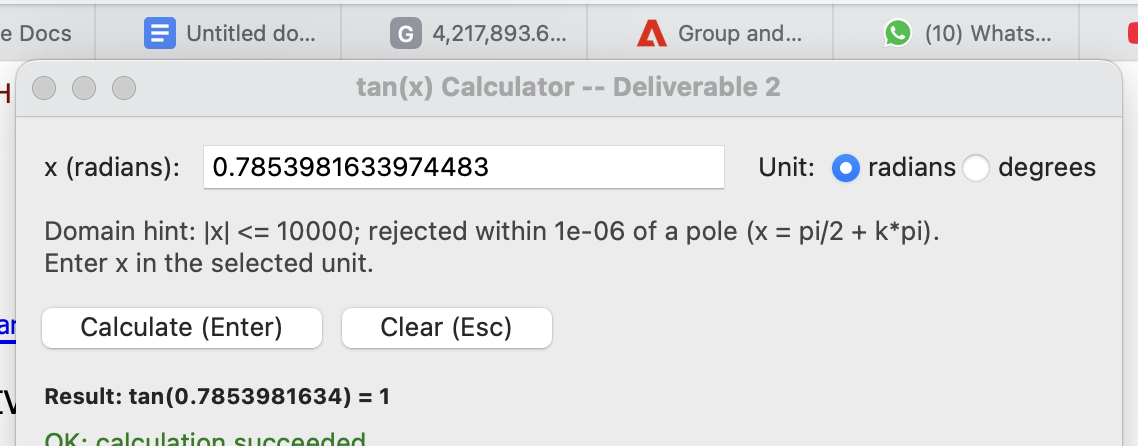
\includegraphics[width=0.85\textwidth]{../../docs/screenshots/d2_gui_valid_pi4.png}\\[0.3cm]
  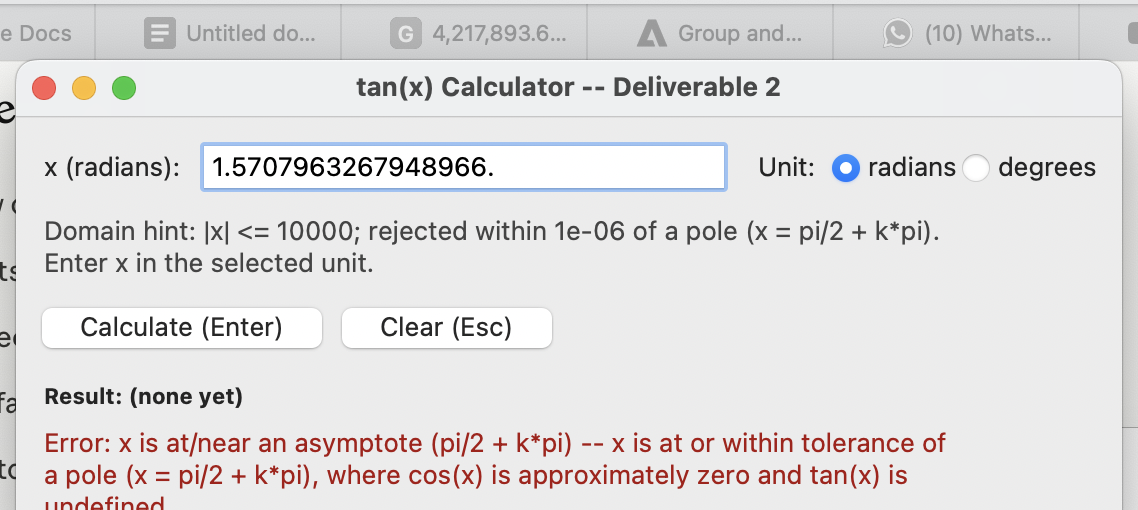
\includegraphics[width=0.85\textwidth]{../../docs/screenshots/d2_gui_near_pole.png}
  \caption{GUI states: valid result for $x=\pi/4$ (top); near-pole rejection at $x=\pi/2$ with a specific, non-colour-only error message (bottom). Three further states (degrees mode, out-of-range, invalid text) are in \texttt{docs/screenshots/}.}
  \label{fig:gui-states}
\end{figure}

\section{Problem 6 --- Repository, Commit History, README}

\subsection{Repository structure}

The repository root now contains \texttt{README.md}, \texttt{src/} (7 modules), \texttt{tests/} (the D2 manual verification script; the graded PyUnit suite is D3), and \texttt{docs/} (persona, requirements v0.1 \emph{and} v0.2, algorithms, decision log, GAI log, the new from-scratch boundary and GUI wireframe docs, and screenshots), matching the task list's suggested layout.

\subsection{Commit history}

D1 was submitted as a Moodle zip before this Git repository was initialized, so it has no incremental history of its own; that limitation is stated honestly in the first commit message rather than hidden or fabricated with backdated commits. From that point forward, D2 work is committed as eleven cohesive, per-concern commits (Table~\ref{tab:commits}) rather than one bulk upload, each with an imperative subject and a body explaining motivation/trade-offs where relevant (D2-P6.2).

\begin{table}[htbp]
\centering
\footnotesize
\begin{tabular}{p{9.5cm}}
\toprule
\textbf{Commit subject (chronological)} \\
\midrule
Add Deliverable 1 baseline: persona, requirements v0.1, algorithms, CLI \\
D2-P5.1: document the from-scratch dependency boundary \\
D2-P5.2/5.3: implement the from-scratch numerical core \\
D2: migrate cli.py onto the shared from-scratch core \\
D2-P5.4: add the Tkinter GUI wireframe \\
D2-P5.5: implement the Tkinter GUI \\
D2-P5.6: add verification suite, capture CLI/GUI evidence \\
D2-P6.3: add project README \\
D2-P7.1: update requirements to baseline v0.2 \\
Log D2 decisions and GAI prompts \\
D2-REP: add D2 LaTeX report and slides \\
\bottomrule
\end{tabular}
\caption{Commit history from repository initialization through this report (\texttt{git log --oneline}).}
\label{tab:commits}
\end{table}

\subsection{README}

\texttt{README.md} states the project's purpose, the from-scratch scope, exact run commands (\texttt{python3 -m src.cli}, \texttt{python3 -m src.gui} --- module invocation, since the package uses absolute \texttt{src.*} imports), usage examples with screenshot references, an error-message/troubleshooting table, the repository structure, and known limitations stated up front (the $10^4$ range bound, the near-pole accuracy margin, and that the formal unit-test suite is a D3 deliverable) rather than only discovered by a reader later.

\section{Problem 7 --- Updated Requirements (Baseline v0.2)}

Every v0.1 requirement was compared against the D2 implementation and \texttt{docs/verification\_matrix\_d2.md}. Table~\ref{tab:changelog} summarizes the changes; 13 v0.1 requirements (FR-01/03/04/05/06, VAL-01--04, ACC-02, USE-01, REL-01/02, ERR-01/02, DOC-01) carry forward \textbf{unchanged} and remain in force.

\begin{table}[htbp]
\centering
\footnotesize
\begin{tabular}{p{1.3cm}p{2cm}p{6.5cm}p{3.5cm}}
\toprule
\textbf{ID} & \textbf{Change} & \textbf{What changed} & \textbf{Discovered via} \\
\midrule
FR-02 & Revised & Angle unit stated \emph{and} selectable (radians default). & Implementation (D-08) \\
FR-07 & New & Labelled degrees input mode. & Implementation (D-08) \\
USE-02 & Revised & "Textual interface" broadened to "at least one interface." & GUI added (D2-P5.5) \\
USE-03 & New & Tkinter GUI with labelled controls, keyboard nav, no colour-only errors. & D2-P5.4/5.5 \\
DEP-01 & New & Core shall not call \texttt{math.sin/cos/tan/pi}. & D2-P5.1/5.2/5.3 \\
ERR-03 & New & Raise one of 3 named exception types, not a bare \texttt{Exception}. & D2 architecture note \\
ACC-01 & Revised (evidence) & Bound unchanged; flagged as tight near the pole boundary ($3.83\times10^{-10}$ measured vs.\ $10^{-9}$ ceiling). & D2-P5.6 verification \\
REL-03 & New & No traceback across 5 documented failure modes (adds convergence). & D2-P5.5/5.6 \\
DOC-02 & New & Document the from-scratch boundary and keep it current. & D2-P5.1 \\
\bottomrule
\end{tabular}
\caption{v0.1 $\to$ v0.2 changelog (full table in \texttt{docs/requirements/requirements\_v0.2.md}).}
\label{tab:changelog}
\end{table}

No requirement was deleted; the v0.1 file is retained on disk unmodified, per constraint C-06 (iterative consistency). ACC-01 was deliberately \emph{not} weakened to make the near-pole margin more comfortable --- it was documented instead, following the same "don't weaken tolerances without justification" principle the task list applies to D3 unit testing.

\section{Verification}
\label{sec:verification}

\texttt{tests/manual\_verification\_d2.py} runs 15 cases against \texttt{math.tan} computed independently (never the from-scratch algorithm verifying itself) --- special angles, odd symmetry, period-$\pi$ reduction, both near-pole directions, both out-of-range directions, and invalid/empty input. All 15 pass within the ACC-01 $10^{-9}$ relative-error bound (Table~\ref{tab:verify}); this is a standalone verification script, not the formal PyUnit suite (D3-P8.2).

\begin{longtable}{L{4cm}L{4.2cm}L{2cm}L{1.3cm}}
\caption{Verification highlights (full 15-case matrix in \texttt{docs/verification\_matrix\_d2.md}).}
\label{tab:verify} \\
\toprule
\textbf{Case} & \textbf{Result} & \textbf{Rel.\ error} & \textbf{Verdict} \\
\midrule
\endhead
$x=\pi/4$ & \small$1.0000000000000013$ & $1.44\times10^{-15}$ & Pass \\
$x=-\pi/4$ (odd symmetry) & \small$-1.0000000000000013$ & $1.44\times10^{-15}$ & Pass \\
$x=\pi+\pi/4$ (period $\pi$) & \small$0.9999999999999996$ & $1.11\times10^{-16}$ & Pass \\
$x=1000$ & \small$1.4703241557018916$ & $5.63\times10^{-13}$ & Pass \\
$x=\pi/2-10^{-6}$ (near pole) & \small$999999.999637844$ & $3.83\times10^{-10}$ & Pass (tightest margin) \\
$x=\pi/2$ (at pole) & raised \texttt{\footnotesize DomainError} & n/a & Pass (rejected) \\
$x=10^{10}$ & raised \texttt{\footnotesize NumericalRangeError} & n/a & Pass (rejected) \\
\texttt{"abc"} / \texttt{""} & raised \texttt{\footnotesize ValueError} & n/a & Pass (rejected) \\
\bottomrule
\end{longtable}

\textbf{Known limitations (honest disclosure):} the $|x|\le10^4$ range bound is unchanged and still provisional pending professor confirmation; the near-pole relative error ($3.83\times10^{-10}$) is the closest margin of any passing case to the $10^{-9}$ ceiling, confirming D1's prediction that precision degrades near the guard-band boundary; no performance/timing requirement is verified (deliberately out of scope).

\section{Decision Rationale}

Key D2 decisions from \texttt{docs/decisions/decision\_log.md}:
\begin{itemize}
  \item \textbf{D-06:} retain Algorithm A rather than switch to CORDIC --- ordinary arithmetic is not prohibited "mathematical support," only library trig calls are, so Algorithm A already satisfies the from-scratch constraint once \texttt{PI} is independently derived.
  \item \textbf{D-07:} derive \texttt{PI} via Machin's arctangent identity rather than a literal digit string, reusing the existing tolerance/max-terms series pattern.
  \item \textbf{D-08:} add an optional, clearly-labelled degrees mode, since the task list explicitly permits it "if time permits" and it directly serves the persona's stated radians/degrees confusion.
\end{itemize}

\section{Implementation Summary}

D2 delivers a fully from-scratch numerical core (Table~\ref{tab:grep}), a Tkinter GUI sharing that core with the CLI, a public version-controlled repository with an eleven-commit incremental history, a README a stranger can run the project from, and a revised requirements baseline (v0.2) with a traceable changelog. All figures, tables, and verification results in this report were produced by the exact source committed as \texttt{D2-REP} in the repository history.

\appendix
\section{GAI Prompt Log (summary)}
\label{sec:gai-log}

Per constraint C-03, the full CASTROFF-informed prompts and evaluation log for Problems 5--7 are in \texttt{docs/prompts/gai\_prompt\_log.md} (D2 section). All three problems used the same tool: Claude Code (Claude, Anthropic, Sonnet 5 model), accessed 2026-07-29. In every case at least one part of the raw output was corrected before being adopted: Problem 5's decision to keep Algorithm A rather than follow D1's own forward-looking note to switch to CORDIC (re-reading the actual from-scratch restriction); the Maclaurin series functions were changed from D1's silent-stop behaviour to raising \texttt{ConvergenceError}, since the D2 architecture note names that exception explicitly; and an early GUI draft that put exception-message formatting inside \texttt{tan\_core.py} was moved out, keeping the numerical core GUI-independent.

\begin{thebibliography}{9}
\bibitem{cooper2007} A. Cooper, R. Reimann, and D. Cronin, \emph{About Face 3: The Essentials of Interaction Design}. Wiley, 2007.
\bibitem{pruitt2006} J. Pruitt and T. Adlin, \emph{The Persona Lifecycle: Keeping People in Mind Throughout Product Design}. Morgan Kaufmann, 2006.
\bibitem{iso29148} ISO/IEC/IEEE, \emph{ISO/IEC/IEEE 29148:2018 -- Systems and Software Engineering -- Life Cycle Processes -- Requirements Engineering}, 2018.
\bibitem{volder1959} J. E. Volder, ``The CORDIC Trigonometric Computing Technique,'' \emph{IRE Transactions on Electronic Computers}, vol. EC-8, no. 3, pp. 330--334, 1959.
\bibitem{muller2016} J.-M. Muller et al., \emph{Handbook of Floating-Point Arithmetic}, 2nd ed. Birkh\"auser, 2016.
\bibitem{machin1706} J. Machin's arctangent identity for $\pi$, as presented in standard numerical-analysis references; see also NIST DLMF below.
\bibitem{abramowitz1964} M. Abramowitz and I. A. Stegun, \emph{Handbook of Mathematical Functions with Formulas, Graphs, and Mathematical Tables}. National Bureau of Standards, 1964.
\bibitem{nist_dlmf} NIST, \emph{NIST Digital Library of Mathematical Functions}, \url{https://dlmf.nist.gov/}, 2026.
\end{thebibliography}

\end{document}
